  \begin{tabular}{l l l l}
    \fbox{{\rd}-1}
    &
    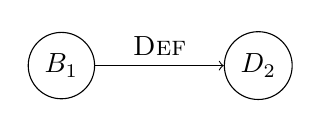
\begin{tikzpicture}[baseline]
      \node [draw,circle] (1) {$B_1$};
      \node [draw,circle,right of=1,xshift=1.5cm] (2) {$D_2$};

      \draw[->] (1) -- node[above] {\textsc{Def}} (2);
    \end{tikzpicture}
    &
    \coloneq
    &
    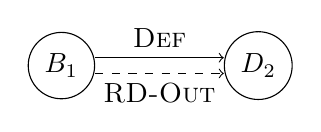
\begin{tikzpicture}[baseline]
      \node [draw,circle] (1) {$B_1$};
      \node [draw,circle,right of=1,xshift=1.5cm] (2) {$D_2$};

      \draw[->,transform canvas={yshift=1mm}] (1) -- node[above] {\textsc{Def}} (2);
      \draw[->,dashed,transform canvas={yshift=-1mm}] (1) -- node[below] {\textsc{RD-Out}} (2);
    \end{tikzpicture}
  \end{tabular}

  \hdash

  \begin{tabular}{l l l l}
    \fbox{{\rd}-2}
    &
    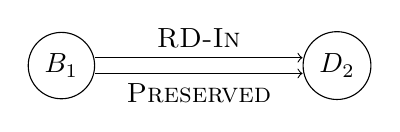
\begin{tikzpicture}[baseline]
      \node [draw,circle] (1) {$B_1$};
      \node [draw,circle,right of=1,xshift=2.5cm] (2) {$D_2$};

      \draw[->,transform canvas={yshift=1mm}] (1) -- node[above] {\textsc{RD-In}} (2);
      \draw[->,transform canvas={yshift=-1mm}] (1) -- node[below] {\textsc{Preserved}} (2);
    \end{tikzpicture}
    &
    \coloneq
    &
    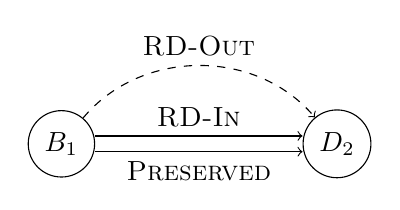
\begin{tikzpicture}[baseline]
      \node [draw,circle] (1) {$B_1$};
      \node [draw,circle,right of=1,xshift=2.5cm] (2) {$D_2$};

      \draw[->,transform canvas={yshift=1mm}] (1) -- node[above] {\textsc{RD-In}} (2);
      \draw[->,transform canvas={yshift=-1mm}] (1) -- node[below] {\textsc{Preserved}} (2);
      \draw[->,dashed] (1) edge[bend left=50] node[above] {\textsc{RD-Out}} (2);
    \end{tikzpicture}
  \end{tabular}

  \hdash

  \begin{tabular}{l l l l}
    \fbox{{\rd}-3}
    &
    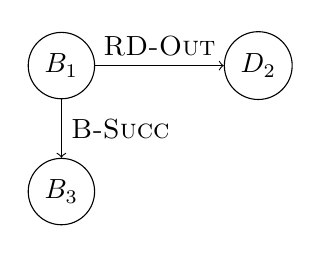
\begin{tikzpicture}[baseline]
      \node [draw,circle] (1) {$B_1$};
      \node [draw,circle,below of=1,yshift=-0.6cm] (3) {$B_3$};
      \node [draw,circle,right of=1,xshift=1.5cm] (2) {$D_2$};

      \draw[->] (1) -- node[right] {\textsc{B-Succ}} (3);
      \draw[->] (1) -- node[above] {\textsc{RD-Out}} (2);
    \end{tikzpicture}
    &
    \coloneq
    &
    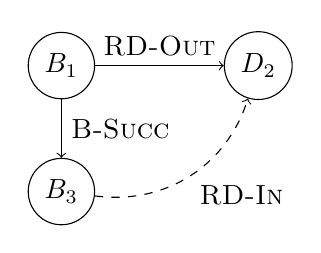
\begin{tikzpicture}[baseline]
      \node [draw,circle] (1) {$B_1$};
      \node [draw,circle,below of=1,yshift=-0.6cm] (3) {$B_3$};
      \node [draw,circle,right of=1,xshift=1.5cm] (2) {$D_2$};

      \draw[->] (1) -- node[right] {\textsc{B-Succ}} (3);
      \draw[->] (1) -- node[above] {\textsc{RD-Out}} (2);
      \draw[->,dashed] (3) edge[bend right=40] node[below right] {\textsc{RD-In}} (2);
    \end{tikzpicture}
  \end{tabular}
